\documentclass[10pt]{article}
\usepackage[polish]{babel}
\usepackage[utf8]{inputenc}
\usepackage[T1]{fontenc}
\usepackage{graphicx}
\usepackage[export]{adjustbox}
\graphicspath{ {./images/} }
\usepackage{amsmath}
\usepackage{amsfonts}
\usepackage{amssymb}
\usepackage[version=4]{mhchem}
\usepackage{stmaryrd}

\title{ARKUSZ PRÓBNEJ MATURY Z OPERONEM MATEMATYKA \\
 POZIOM PODSTAWOWY }

\author{}
\date{}


\begin{document}
\maketitle
\section*{Czas pracy: 170 minut}
\section*{Instrukcja dla zdającego}
\begin{enumerate}
  \item Sprawdź, czy arkusz egzaminacyjny zawiera 19 stron (zadania 1.-35.). Ewentualny brak zgłoś przewodniczącemu zespołu nadzorującego egzamin.
  \item Rozwiązania zadań i odpowiedzi zapisz w miejscu na to przeznaczonym.
  \item W zadaniach zamkniętych (1.-28.) zaznacz jedną poprawną odpowiedź.
  \item W rozwiązaniach zadań otwartych (29.-35.) przedstaw tok rozumowania prowadzący do ostatecznego wyniku.
  \item Pisz czytelnie. Używaj długopisu/pióra tylko z czarnym tuszem/atramentem.
  \item Nie używaj korektora, a błędne zapisy wyraźnie przekreśl.
  \item Zapisy w brudnopisie nie będą oceniane.
  \item Obok numeru każdego zadania podana jest maksymalna liczba punktów możliwych do uzyskania.
  \item Możesz korzystać z zestawu wzorów matematycznych, cyrkla i linijki oraz kalkulatora prostego.
\end{enumerate}

Za rozwiązanie wszystkich zadań można otrzymać\\
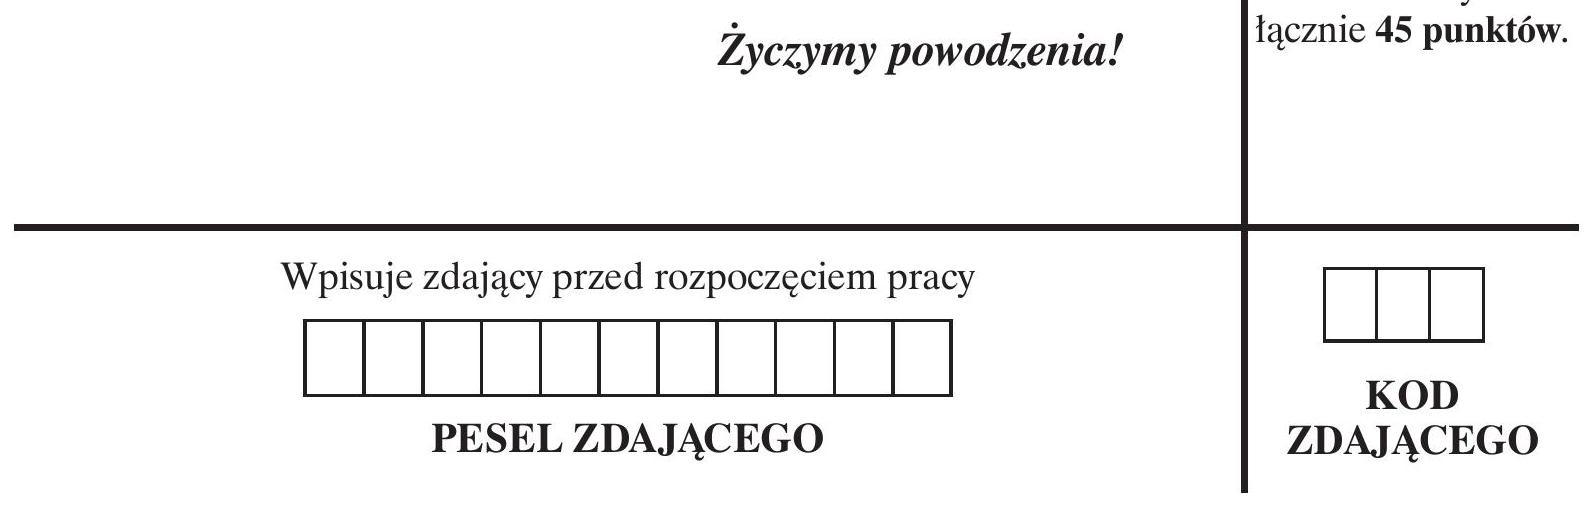
\includegraphics[max width=\textwidth, center]{2024_11_21_cdea326d19d0c2132b88g-01}

Arkusz opracowany przez Wydawnictwo Pedagogiczne OPERON.\\
Kopiowanie w całości lub we fragmentach bez zgody wydawcy zabronione.

\section*{ZADANIA ZAMKNIĘTE}
W zadaniach od 1. do 28. wybierz i zaznacz jedną poprawną odpowiedź.

\section*{Zadanie 1. (0-1)}
Wyrażenie \(\frac{10^{13} \cdot 7^{13}}{14^{13} \cdot 5^{10}}\) jest równe:\\
A. \(7^{2}\)\\
B. \(2^{10}\)\\
C. \(5^{3}\)\\
D. \(10^{5}\)

\section*{Zadanie 2. (0-1)}
Liczbą odwrotną do liczby \(\frac{1+\sqrt{3}}{2}\) jest liczba:\\
A. \(-\frac{1+\sqrt{3}}{2}\)\\
B. \(3 \sqrt{3}+1\)\\
C. \(\frac{3-\sqrt{3}}{2}\)\\
D. \(\sqrt{3}-1\)

\section*{Zadanie 3. (0-1)}
Najmniejsza wartość wyrażenia \((x-y)(x+y)\) dla \(x, y \in\{2,3,4\}\) jest równa:\\
A. -12\\
B. 0\\
C. 2\\
D. 24

\section*{Zadanie 4. (0-1)}
Laptop kosztował 1500 zł. Jego cenę obniżono o 20\%, a następnie podwyższono o 20\%. Po tych operacjach laptop kosztuje:\\
A. 1500 zt\\
B. 1440 zf\\
C. \(1550 \mathrm{zł}\)\\
D. \(1600 \mathrm{zł}\)

\section*{Zadanie 5. (0-1)}
Wartość wyrażenia \(3 \log _{4} 2+\log _{4} 32\) jest równa:\\
A. 1\\
B. 2\\
C. 3\\
D. 4

\section*{Zadanie 6. (0-1)}
Największą liczbą całkowitą spełniającą nierówność \(\sqrt{2}-\frac{x}{3} \geq 0\) jest:\\
A. \(-3 \sqrt{2}\)\\
B. 4\\
C. \(3 \sqrt{2}\)\\
D. -4

\section*{Zadanie 7. (0-1)}
Suma pierwiastków równania \(x\left(x^{2}+16\right)(x-11)(x+12)=0\) wynosi:\\
A. 1\\
B. 2\\
C. -1\\
D. -2

\section*{BRUDNOPIS (nie podlega ocenie)}
\begin{center}

\includegraphics[max width=\textwidth]{2024_11_21_cdea326d19d0c2132b88g-03}
\end{center}

\section*{Zadanie 8. (0-1)}
Wykresem funkcji kwadratowej \(f(x)=-2(x+3)^{2}-4\) jest parabola, a osią symetrii tej paraboli jest prosta o równaniu:\\
A. \(x=3\)\\
B. \(x=-3\)\\
C. \(x=4\)\\
D. \(x=-4\)

\section*{Zadanie 9. (0-1)}
Funkcja liniowa \(f(x)=(m-\sqrt{2}) x+11\) jest rosnąca dla:\\
A. \(m \geq \sqrt{2}\)\\
B. \(m \leq \sqrt{2}\)\\
C. \(m<\sqrt{2}\)\\
D. \(m>\sqrt{2}\)

\section*{Zadanie 10. (0-1)}
Prostą równoległą do prostej \(k: 3 x+2 y-5=0\), przechodzącą przez punkt \(P=(2,-5)\), jest prosta:\\
A. \(l: y=-\frac{3}{2} x-2\)\\
B. \(l: y=\frac{3}{2} x-2\)\\
C. \(l: y=-\frac{3}{2} x+2\)\\
D. \(l: y=\frac{3}{2} x+2\)

\section*{Zadanie 11. (0-1)}
Wierzchołkiem paraboli będącej wykresem funkcji \(f(x)=3 x^{2}-30 x+82\) jest punkt:\\
A. \(W=(-5,7)\)\\
B. \(W=(5,-7)\)\\
C. \(W=(5,7)\)\\
D. \(W=(-5,-7)\)

\section*{Zadanie 12. (0-1)}
W rosnącym ciągu arytmetycznym spełniony jest warunek \(a_{3}+a_{7}=28\), więc:\\
A. \(a_{5}=14\)\\
B. \(a_{5}=7\)\\
C. \(a_{5}=21\)\\
D. \(a_{5}=12\)

\section*{Zadanie 13. (0-1)}
Dany jest trzywyrazowy ciąg geometryczny \((3,6,5 x+2)\). Zatem:\\
A. \(x=-6\)\\
B. \(x=2\)\\
C. \(x=6\)\\
D. \(x=-2\)

\section*{Zadanie 14. (0-1)}
W ciągu liczbowym \(a_{n}=(-1)^{2 n+1} \cdot\left(2^{n-1}-1\right)\) dla \(n \geq 1\) suma \(a_{5}+a_{11}\) jest równa:\\
A. 1024\\
B. 1038\\
C. -1024\\
D. -1038

\section*{BRUDNOPIS (nie podlega ocenie)}
\begin{center}

\includegraphics[max width=\textwidth]{2024_11_21_cdea326d19d0c2132b88g-05}
\end{center}

\section*{Zadanie 15. (0-1)}
Zbiorem wartości funkcji, której wykres przedstawiono na rysunku, jest zbiór:\\
A. \((-6,3)\)\\
B. \((-6,6)\)\\
C. \(\langle-6,3)\)\\
D. \(\langle-6,3\rangle\)\\
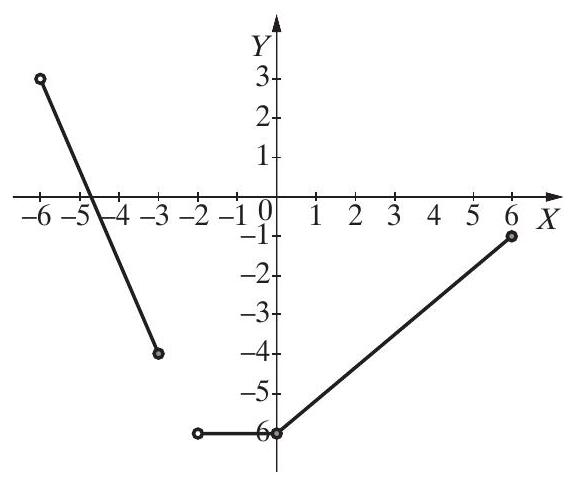
\includegraphics[max width=\textwidth, center]{2024_11_21_cdea326d19d0c2132b88g-06}

\section*{Zadanie 16. (0-1)}
Miara kąta wewnętrznego wielokąta foremnego wynosi \(156^{\circ}\). Ten wielokąt, to:\\
A. dziesięciokąt\\
B. dwunastokąt\\
C. piętnastokąt\\
D. dwudziestokąt

\section*{Zadanie 17. (0-1)}
Zaznaczone na rysunku kąty \(\alpha, \beta, \gamma\) mają miary:\\
A. \(\alpha=60^{\circ}, \beta=30^{\circ}, \gamma=30^{\circ}\)\\
B. \(\alpha=50^{\circ}, \beta=40^{\circ}, \gamma=40^{\circ}\)\\
C. \(\alpha=70^{\circ}, \beta=20^{\circ}, \gamma=20^{\circ}\)\\
D. \(\alpha=30^{\circ}, \beta=60^{\circ}, \gamma=60^{\circ}\)

\section*{Zadanie 18. (0-1)}
\begin{center}
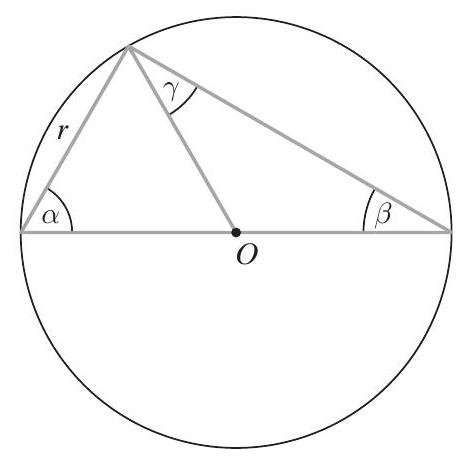
\includegraphics[max width=\textwidth]{2024_11_21_cdea326d19d0c2132b88g-06(2)}
\end{center}

Pole trapezu równoramiennego o wysokości 5 jest równe 45. Odcinek łączący środki ramion tego trapezu ma długość:\\
A. \(5 \sqrt{3}\)\\
B. \(9 \sqrt{3}\)\\
C. 10\\
D. 9

\section*{Zadanie 19. (0-1)}
W trójkącie \(K L M\) punkt \(A\) leży na boku \(K M\), a punkt \(B\) leży na boku \(L M\). Odcinek \(A B\) jest równoległy do boku \(K L\) oraz \(|K L|=9,|K A|=3,|A B|=4\) (zobacz rysunek).\\
Odcinek \(A M\) ma długość:\\
A. 3,6\\
B. 2,4\\
C. 3\\
D. 1,8\\
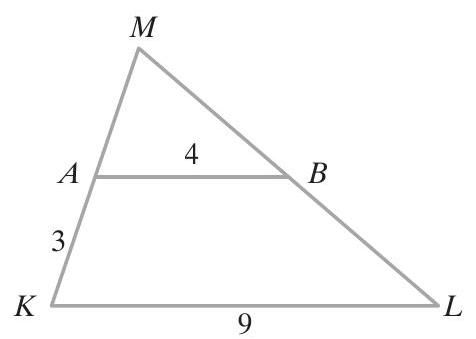
\includegraphics[max width=\textwidth, center]{2024_11_21_cdea326d19d0c2132b88g-06(1)}

\section*{Zadanie 20. (0-1)}
Wartość wyrażenia \(\left(\operatorname{tg} \alpha-\operatorname{tg}^{2} \alpha\right) \cdot \cos \alpha\) dla kąta ostrego \(\alpha\), dla którego \(\sin \alpha=\frac{3}{5}\), wynosi:\\
A. \(\frac{16}{25}\)\\
B. \(\frac{3}{10}\)\\
C. \(\frac{3}{20}\)\\
D. \(\frac{1}{10}\)

\section*{BRUDNOPIS (nie podlega ocenie)}
\begin{center}

\includegraphics[max width=\textwidth]{2024_11_21_cdea326d19d0c2132b88g-07}
\end{center}

\section*{Zadanie 21. (0-1)}
Punkty \(A=(3,-2)\) i \(C=(-2,3)\) są przeciwległymi wierzchołkami kwadratu \(A B C D\).\\
Obwód tego kwadratu jest równy:\\
A. \(25 \sqrt{6}\)\\
B. \(5 \sqrt{2}\)\\
C. \(10 \sqrt{3}\)\\
D. 20

\section*{Zadanie 22. (0-1)}
Objętość sześcianu, którego suma długości krawędzi jest równa 72, wynosi:\\
A. 216\\
B. 160\\
C. 36\\
D. 240

\section*{Zadanie 23. (0-1)}
Objętość prostopadłościanu, którego każda następna krawędź jest dwa razy dłuższa od poprzedniej, wynosi 216. Pole powierzchni tego prostopadłościanu jest równe:\\
A. 126\\
B. 252\\
C. 522\\
D. 110

\section*{Zadanie 24. (0-1)}
Przekątna graniastosłupa prawidłowego czworokatnego o długości \(d\) jest nachylona do płaszczyzny podstawy pod kątem \(\alpha\) takim, że \(\sin \alpha=\frac{\sqrt{2}}{2}\). Objętość tego graniastosłupa wyraża się wzorem:\\
A. \(\frac{\sqrt{2}}{2} d^{3}\)\\
B. \(\frac{\sqrt{2}}{4} d^{3}\)\\
C. \(\frac{\sqrt{2}}{8} d^{3}\)\\
D. \(\frac{\sqrt{2}}{10} d^{3}\)

\section*{Zadanie 25. (0-1)}
Na diagramie słupkowym przedstawiono oceny końcowe ucznia.\\
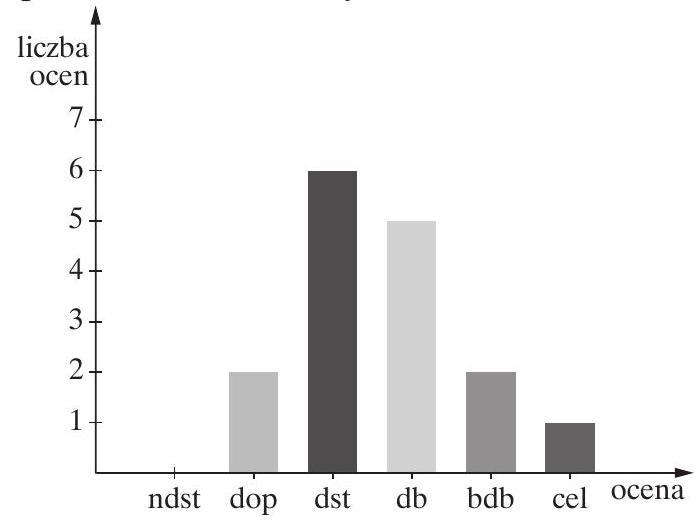
\includegraphics[max width=\textwidth, center]{2024_11_21_cdea326d19d0c2132b88g-08}

Mediana ocen ucznia jest równa:\\
A. 3\\
B. 3,5\\
C. 4\\
D. 4,5

\section*{Zadanie 26. (0-1)}
Mediana zestawu danych: 1, 1, 2, 2, x, 4, 6, 7, 9, 11, wynosi 3,5.\\
Zatem średnia arytmetyczna tego zestawu jest równa:\\
A. 4,6\\
B. 6,5\\
C. 7,25\\
D. 8,75

\section*{BRUDNOPIS (nie podlega ocenie)}
\begin{center}

\includegraphics[max width=\textwidth]{2024_11_21_cdea326d19d0c2132b88g-09}
\end{center}

\section*{Zadanie 27. (0-1)}
Wyniki dwukrotnego rzutu sześcienną kostką do gry zapisujemy jako liczby dwucyfrowe. Prawdopodobieństwo otrzymania liczby podzielnej przez 4 wynosi:\\
A. \(\frac{1}{3}\)\\
B. \(\frac{1}{4}\)\\
C. \(\frac{3}{4}\)\\
D. \(\frac{2}{3}\)

\section*{Zadanie 28. (0-1)}
Rzucamy dwa razy monetą i dwa razy sześcienną kostką do gry. Wyniki zapisujemy w kolejności rzutów: moneta, moneta, kostka, kostka. Prawdopodobieństwo otrzymania dokładnie dwóch orłów i tych samych liczb oczek wynosi:\\
A. \(\frac{1}{24}\)\\
B. \(\frac{1}{72}\)\\
C. \(\frac{1}{6}\)\\
D. \(\frac{1}{12}\)

\section*{BRUDNOPIS (nie podlega ocenie)}
\begin{center}

\includegraphics[max width=\textwidth]{2024_11_21_cdea326d19d0c2132b88g-11}
\end{center}

\section*{ZADANIA OTWARTE}
Rozwiązania zadań 29.-35. należy zapisać w wyznaczonych miejscach pod treścią zadania.

\section*{Zadanie 29. (0-2)}
Rozwiąż nierówność \((x-1)^{2} \leq \frac{3}{2}\).\\

\includegraphics[max width=\textwidth, center]{2024_11_21_cdea326d19d0c2132b88g-12}

Odpowiedź: \(\qquad\)\\
12

Zadanie 30. (0-2)\\
Uzasadnij, że dla każdej dodatniej liczby naturalnej \(n\) liczba \(4^{n+1}-3^{n+2}+4^{n}-3^{n}\) jest podzielna przez 5.\\

\includegraphics[max width=\textwidth, center]{2024_11_21_cdea326d19d0c2132b88g-13}

\section*{Zadanie 31. (0-2)}
Suma sześciu początkowych wyrazów ciągu arytmetycznego wynosi 72, a szósty wyraz tego ciągu jest równy 22. Oblicz pierwszy wyraz tego ciągu.\\

\includegraphics[max width=\textwidth, center]{2024_11_21_cdea326d19d0c2132b88g-14}

Odpowiedź:

14

\section*{Zadanie 32. (0-2)}
Oblicz miary kątów równoległoboku o bokach długości 5 i 12 oraz o polu równym 30.\\

\includegraphics[max width=\textwidth, center]{2024_11_21_cdea326d19d0c2132b88g-15}

Odpowiedź:

\section*{Zadanie 33. (0-2)}
Przekątna \(A C\) rombu \(A B C D\) o wierzchołkach \(A(-7,2), B(5,-3)\) ma długość 24 . Oblicz długość przekątnej \(B D\) tego rombu.\\

\includegraphics[max width=\textwidth, center]{2024_11_21_cdea326d19d0c2132b88g-16}

Odpowiedź: \(\qquad\)\\
16

\section*{Zadanie 34. (0-3)}
Krawędzie prostopadłościanu wychodzące z jednego wierzchołka mają długości będące kolejnymi liczbami nieparzystymi. Suma długości wszystkich krawędzi tego prostopadłościanu wynosi 60 . Oblicz objętość i pole powierzchni tej bryły.\\

\includegraphics[max width=\textwidth, center]{2024_11_21_cdea326d19d0c2132b88g-17}

Odpowiedź: \(\qquad\)

\section*{Zadanie 35. (0-4)}
Funkcja kwadratowa \(f(x)=a x^{2}+b x+c\) ma dwa miejsca zerowe \(x_{1}=-2 \frac{1}{2}\) i \(x_{2}=1\). Wykres funkcji \(f\) przechodzi przez punkt \(A(-3,8)\). Wyznacz najmniejszą wartość funkcji \(f\).

\begin{center}
\begin{tabular}{|c|c|c|c|c|c|c|c|c|c|c|c|c|c|c|c|c|c|c|c|c|c|c|c|}
\hline
 &  &  &  &  &  &  &  &  &  &  &  &  &  &  &  &  &  &  &  &  &  &  &  \\
\hline
 &  &  &  &  &  &  &  &  &  &  &  &  &  &  &  &  &  &  &  &  &  &  &  \\
\hline
 &  &  &  &  &  &  &  &  &  &  &  &  &  &  &  &  &  &  &  &  &  &  &  \\
\hline
 &  &  &  &  &  &  &  &  &  &  &  &  &  &  &  &  &  &  &  &  &  &  &  \\
\hline
 &  &  &  &  &  &  &  &  &  &  &  &  &  &  &  &  &  &  &  &  &  &  &  \\
\hline
 &  &  &  &  &  &  &  &  &  &  &  &  &  &  &  &  &  &  &  &  &  &  &  \\
\hline
 &  &  &  &  &  &  &  &  &  &  &  &  &  &  &  &  &  &  &  &  &  &  &  \\
\hline
 &  &  &  &  &  &  &  &  &  &  &  &  &  &  &  &  &  &  &  &  &  &  &  \\
\hline
 &  &  &  &  &  &  &  &  &  &  &  &  &  &  &  &  &  &  &  &  &  &  &  \\
\hline
 &  &  &  &  &  &  &  &  &  &  &  &  &  &  &  &  &  &  &  &  &  &  &  \\
\hline
 &  &  &  &  &  &  &  &  &  &  &  &  &  &  &  &  &  &  &  &  &  &  &  \\
\hline
 &  &  &  &  &  &  &  &  &  &  &  &  &  &  &  &  &  &  &  &  &  &  &  \\
\hline
 &  &  &  &  &  &  &  &  &  &  &  &  &  &  &  &  &  &  &  &  &  &  &  \\
\hline
 &  &  &  &  &  &  &  &  &  &  &  &  &  &  &  &  &  &  &  &  &  &  &  \\
\hline
 &  &  &  &  &  &  &  &  &  &  &  &  &  &  &  &  &  &  &  &  &  &  &  \\
\hline
 &  &  &  &  &  &  &  &  &  &  &  &  &  &  &  &  &  &  &  &  &  &  &  \\
\hline
 &  &  &  &  &  &  &  &  &  &  &  &  &  &  &  &  &  &  &  &  &  &  &  \\
\hline
 &  &  &  &  &  &  &  &  &  &  &  &  &  &  &  &  &  &  &  &  &  &  &  \\
\hline
 &  &  &  &  &  &  &  &  &  &  &  &  &  &  &  &  &  &  &  &  &  &  &  \\
\hline
 &  &  &  &  &  &  &  &  &  &  &  &  &  &  &  &  &  &  &  &  &  &  &  \\
\hline
 &  &  &  &  &  &  &  &  &  &  &  &  &  &  &  &  &  &  &  &  &  &  &  \\
\hline
 &  &  &  &  &  &  &  &  &  &  &  &  &  &  &  &  &  &  &  &  &  &  &  \\
\hline
 &  &  &  &  &  &  &  &  &  &  &  &  &  &  &  &  &  &  &  &  &  &  &  \\
\hline
 &  &  &  &  &  &  &  &  &  &  &  &  &  &  &  &  &  &  &  &  &  &  &  \\
\hline
 &  &  &  &  &  &  &  &  &  &  &  &  &  &  &  &  &  &  &  &  &  &  &  \\
\hline
 &  &  &  &  &  &  &  &  &  &  &  &  &  &  &  &  &  &  &  &  &  &  &  \\
\hline
 &  &  &  &  &  &  &  &  &  &  &  &  &  &  &  &  &  &  &  &  &  &  &  \\
\hline
 &  &  &  &  &  &  &  &  &  &  &  &  &  &  &  &  &  &  &  &  &  &  &  \\
\hline
 &  &  &  &  &  &  &  &  &  &  &  &  &  &  &  &  &  &  &  &  &  &  &  \\
\hline
 &  &  &  &  &  &  &  &  &  &  &  &  &  &  &  &  &  &  &  &  &  &  &  \\
\hline
 &  &  &  &  &  &  &  &  &  &  &  &  &  &  &  &  &  &  &  &  &  &  &  \\
\hline
 &  &  &  &  &  &  &  &  &  &  &  &  &  &  &  &  &  &  &  &  &  &  &  \\
\hline
 &  &  &  &  &  &  &  &  &  &  &  &  &  &  &  &  &  &  &  &  &  &  &  \\
\hline
 &  &  &  &  &  &  &  &  &  &  &  &  &  &  &  &  &  &  &  &  &  &  &  \\
\hline
 &  &  &  &  &  &  &  &  &  &  &  &  &  &  &  &  &  &  &  &  &  &  &  \\
\hline
 &  &  &  &  &  &  &  &  &  &  &  &  &  &  &  &  &  &  &  &  &  &  &  \\
\hline
 &  &  &  &  &  &  &  &  &  &  &  &  &  &  &  &  &  &  &  &  &  &  &  \\
\hline
 &  &  &  &  &  &  &  &  &  &  &  &  &  &  &  &  &  &  &  &  &  &  &  \\
\hline
 &  &  &  &  &  &  &  &  &  &  &  &  &  &  &  &  &  &  &  &  &  &  &  \\
\hline
 &  &  &  &  &  &  &  &  &  &  &  &  &  &  &  &  &  &  &  &  &  &  &  \\
\hline
 &  &  &  &  &  &  &  &  &  &  &  &  &  &  &  &  &  &  &  &  &  &  &  \\
\hline
\end{tabular}
\end{center}

Odpowiedź: \(\qquad\)\\
18

\section*{BRUDNOPIS (nie podlega ocenie)}

\includegraphics[max width=\textwidth, center]{2024_11_21_cdea326d19d0c2132b88g-19}\\
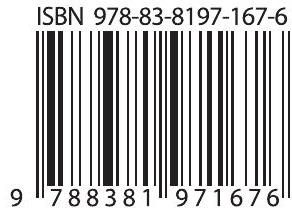
\includegraphics[max width=\textwidth, center]{2024_11_21_cdea326d19d0c2132b88g-20}


\end{document}